%!TEX encoding = UTF-8 Unicode

%\documentclass{report}
%\usepackage[cjk]{kotex}

\documentclass{memoir}
\usepackage[cjk]{kotex}


%\usepackage{ikps,ansform}
\usepackage{amsthm}
\usepackage{thmtools}
\usepackage{lipsum}
\usepackage{url}
\usepackage{amsmath}
\usepackage{amssymb}
%\usepackage{ansform}
\usepackage{thmtools}
\usepackage{graphicx}
%https://www.overleaf.com/learn/latex/Inserting_Images

\usepackage{listings}
\usepackage{xcolor}
\declaretheoremstyle[% spaceabove=6pt,spacebelow=6pt, headfont=\color{MainColorOne}\sffamily\bfseries, notefont=\mdseries, notebraces={[}{]}, bodyfont=\normalfont,
headpunct={},
postheadspace=1em,
%qed=▣,
]{maintheorem}

\declaretheorem[%
name=정의,
style=maintheorem,
numberwithin=chapter, shaded={%bgcolor=MainColorThree!20,
margin=.5em}]{dfn}
% \begin{dfn}[]
% \end{dfn}

\newtheorem{theorem}{Theorem}[chapter]
\newtheorem{corollary}{Corollary}[theorem]
\newtheorem{lemma}[theorem]{Lemma}
%https://www.overleaf.com/learn/latex/Theorems_and_proofs

\definecolor{mGreen}{rgb}{0,0.6,0}
\definecolor{mGray}{rgb}{0.5,0.5,0.5}
\definecolor{mPurple}{rgb}{0.58,0,0.82}
\definecolor{backgroundColour}{rgb}{0.95,0.95,0.92}
%https://tex.stackexchange.com/questions/348651/c-code-to-add-in-the-document
\lstdefinestyle{CStyle}{
    backgroundcolor=\color{backgroundColour},   
    commentstyle=\color{mGreen},
    keywordstyle=\color{magenta},
    numberstyle=\tiny\color{mGray},
    stringstyle=\color{mPurple},
    basicstyle=\footnotesize,
    breakatwhitespace=false,         
    breaklines=true,                 
    captionpos=b,                    
    keepspaces=true,                 
    numbers=left,                    
    numbersep=5pt,                  
    showspaces=false,                
    showstringspaces=false,
    showtabs=false,                  
    tabsize=2,
    language=C
}
\usepackage{bookmark}

\bookmarksetup{startatroot}


\begin{document}
    
\title{CSAPP}
\author{ EUnS }

\maketitle

\tableofcontents



\chapter{Concurrent Programming}

동시성 프로그래밍을 하는 경우.

\begin{itemize}
    \item Accessing slow I/O devices
    \item Interacting with humans.
    \item Reducing latency by deferring work
    \item Servicing multiple network clients
    \item Computing in parallel on multi-core machines
\end{itemize}

동시성 프로그램을 위한 세가지 접근 방법
\begin{itemize}
    \item Processes
    \item I/O multiplexing
    \item Threads
\end{itemize}



\section{Concurrent Programming with Processes}
A Concurrent Server Based on Processes
Pros and Cons of Processes

pork exec, waitpid등의 프로세스 제어 함수를 사용한다
특징
\begin{itemize}
    \item 분리된 주소공간을 가진다.
    \item 프로세스가 상태정보를 공유하는것이 어렵다.
    \item 명시적인 IPC(interprocess communications)를 사용해야한다..
    \item 프로세스 제어와 IPC 오버헤드가 크기 때문에 더 느려질수있다.
\end{itemize}


\section{Concurrent Programming with I/O Multiplexing}
1 A Concurrent Event-Driven Server Based on I/Multiplexing
2 Pros and Cons of I/O Multiplexing




\section{Concurrent Programming with Threads}
1 Thread Execution Model
2 Posix Threads
3 Creating Threads
4 Terminating Threads
5 Reaping Terminated Threads
6 Detaching Threads
7 Initializing Threads
8 A Concurrent Server Based on Threads
Shared Variables in Threaded Programs
1 Threads Memory Model
2 Mapping Variables to Memory
3 Shared Variables
Synchronizing Threads with Semaphores
1 Progress Graphs
2 Semaphores
3 Using Semaphores for Mutual Exclusion
4 Using Semaphores to Schedule Shared Resources
5 Putting It Together: A Concurrent Server Based Prethreading
Using Threads for Parallelism




Other Concurrency Issues
1 Thread Safety
2 Reentrancy
3 Using Existing Library Functions in Threaded Programs
4 Races
5 Deadlocks
Summary



\chapter{Machine-Level Representation of Programs}


linux> gcc -Og -o p p1.c p2.c


-0g 옵션 : 최적화 x

ISA (instruction set architectune)

linux> gcc -Og -S mstore.c

-S : 어셈블리 코드만 만든다 .s

linux> gcc -Og -c mstore.c

바이너리 형식 목적파일 .o  생성


linux> objdump -d mstore.o

disassembly


\section{x86 assembly}


% \begin{figure}[h!]
%     \centering
% %    \includegraphics[scale=0.5]{pic/section12/pit1}
%     \caption{ward 0x1234567이 저장되는 방식.}
% \end{figure}




% \begin{figure}[h!]
%     \centering
%     \includegraphics[scale=0.5]{pic/section12/pit1}
%     \caption{ward 0x1234567이 저장되는 방식.}
% \end{figure}





3.1 A Historical Perspective 202
3.2 Program Encodings 205
3.3 Data Formats 213
3.4 Accessing Information 215
3.5 Arithmetic and Logical Operations 227
3.6 Control 236
3.7 Procedures 274
3.8 Array Allocation and Access 291
3.9 Heterogeneous Data Structures 301
3.10 Combining Control and Data in Machine-Level Programs 312
3.11 Floating-Point Code 329
3.12 Summary 345

\chapter{Processor Architecture}

387
4.1 The Y86-64 Instruction Set Architecture 391
4.2 Logic Design and the Hardware Control Language HCL 408
4.3 Sequential Y86-64 Implementations 420
4.4 General Principles of Pipelining 448
4.5 Pipelined Y86-64 Implementations 457
4.6 Summary 506
4.6.1 Y86-64 Simulators 508
Bibliographic Notes 509
Homework Problems 509
Solutions to Practice Problems 516



\chapter{Optimizing Program Performance}

\begin{enumerate}
    \item select an appropriate set of algorithms and data structures
    \item  write source code that the compiler can effectively optimize to turn into efficient executable code
    \item  divide a task into portions that can be computed in parallel, on some combination of multiple cores and multiple processors.
\end{enumerate}
명심할것. 두번째를 이해하기위해 컴파일러의 능력과 한계를 알아야한다. 최적화를 위하면서도 코드 가독성은 유지해야한다.


\section{Capabilities and Limitations of Optimizing Compilers}


컴파일러 최적화 명령어는 -0g -1g -2g ... 이 있다.


다음 두개의 코드가 있다고 생각해보자 
\begin{lstlisting}[style = CStyle]
void twiddle1(long *xp, long *yp)
{
*xp += *yp;
*xp += *yp;
}

void twiddle2(long *xp, long *yp)
{
*xp += 2* *yp;
}
\end{lstlisting}
twiddle1은 twiddle2로 최적화 될수있는가? 답은 아니 다. xp와 yp가 동일하다고 생각해보자. 그러면 명확할 것이다.


\begin{lstlisting}[style = CStyle]
long f();
long func1() {
return f() + f() + f() + f();
}

long func2() {
return 4*f();
}
\end{lstlisting}
func1 이 func2로 최적화 될 수 있다고 생각한다. 하지만 f에서 전역변수를 건든다고 생각해보자 4번 바뀔게 한번만 바뀌는 일이 될것이다.

컴파일러는 위험요소가 있을경우 최적화를 하지않는다.

\section{Eliminating Loop Inefficiencies}

\begin{lstlisting}[style = CStyle]
void combine1(vec_ptr v, data_t *dest)
 {
 long i;

 *dest = IDENT;
 for (i = 0; i < vec_length(v); i++) {
 data_t val;
 get_vec_element(v, i, &val);
 *dest = *dest OP val;
 }
 }

\end{lstlisting}

이게 어떻게 성능 개선이되는지 보자.

\begin{lstlisting}[style = CStyle]
void combine2(vec_ptr v, data_t *dest)
 {
 long i;
 long length = vec_length(v);

 *dest = IDENT;
 for (i = 0; i < length; i++) {
 data_t val;
 get_vec_element(v, i, &val);
 *dest = *dest OP val;
 }
 }
\end{lstlisting}


\begin{figure}[h!]
    \centering
    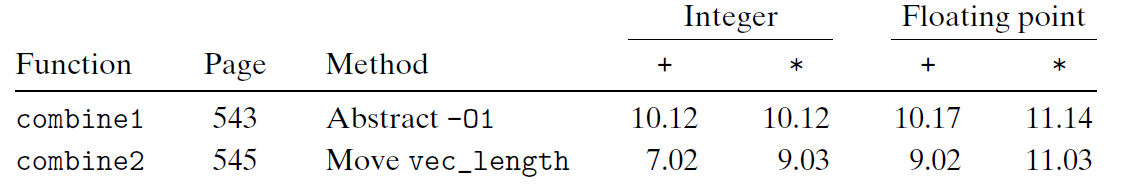
\includegraphics[scale=0.4]{pic/section5/pic1}
\end{figure}



\begin{lstlisting}[style = CStyle]
/* Convert string to lowercase: slow */
void lower1(char *s)
{
    long i;

    for (i = 0; i < strlen(s); i++)
        if (s[i] >= `A' && s[i] <= 'Z')
            s[i] -= ('A' - 'a');    
}

/* Convert string to lowercase: faster */
void lower2(char *s)
{
    long i;
    long len = strlen(s);

    for (i = 0; i < len; i++)
        if (s[i] >= `A' && s[i] <= 'Z')
            s[i] -= (`A' - 'a');
}

/* Sample implementation of library function strlen */
/* Compute length of string */
size_t strlen(const char *s)
{
    long length = 0;
    while (*s != '\0') {
        s++;
        length++;
    }
    return length;
}
\end{lstlisting}

\begin{figure}[h!]
    \centering
    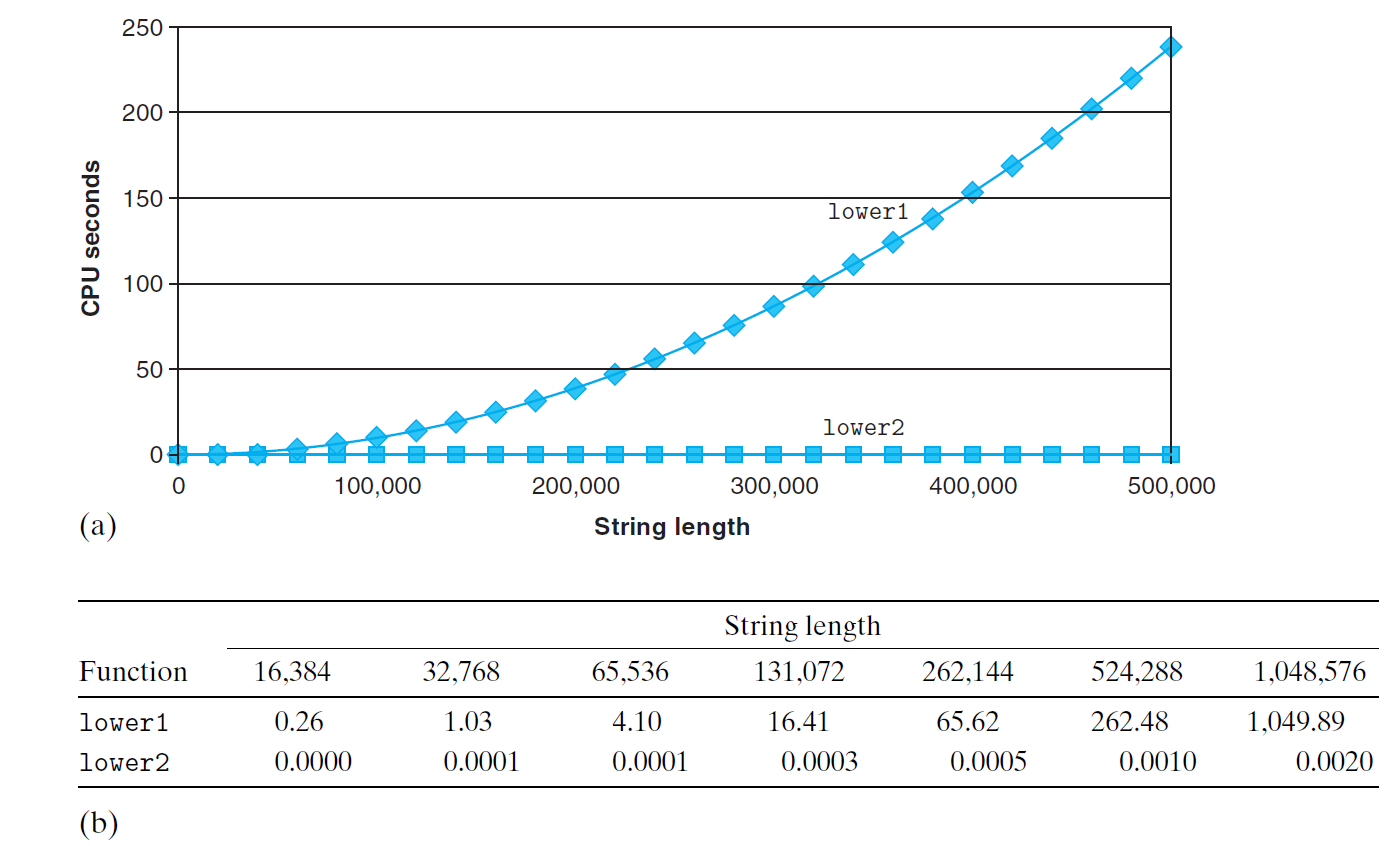
\includegraphics[scale=0.4]{pic/section5/pic2}
    \caption{lower 성능비교}
\end{figure}

시간복잡도 계산으로도 충분히 알 수 있다.
문자열 길이가 변하는게 아니라면 strlen을 반복문안에 넣는 짓은 하지말자.

\section{Reducing Procedure Calls}

\begin{lstlisting}[style = CStyle]
void combine3(vec_ptr v, data_t *dest)
{
    long i;
    long length = vec_length(v);
    data_t *data = get_vec_start(v);
    *dest = IDENT;
    for (i = 0; i < length; i++) {
    *dest = *dest OP data[i];
    }
}
\end{lstlisting}

대충 함수안에서 계속 함수를 쳐부르는 짓은 오버헤드와 불리는 함수안에서 처리하는 불필요한 작업으로 느려진다는 뜻.
근데 뒤에 더다룬다함


\begin{figure}[h!]
    \centering
    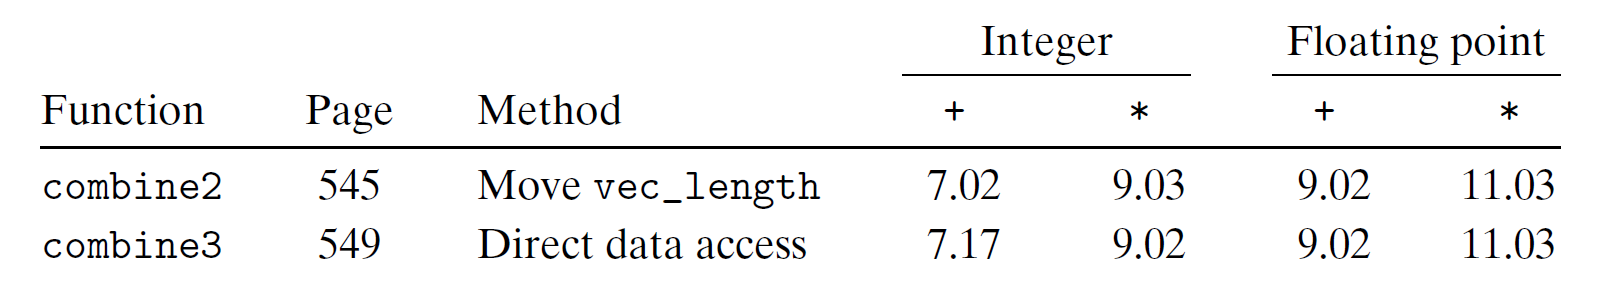
\includegraphics[scale=0.3]{pic/section5/pic3}
\end{figure}

\section{Eliminating Unneeded Memory References}

combine3에서 내부 루프는 포인터 dest가 메모리 참조를 계속하는 식이다.
다음 방식이 조금더 효율적이다.

\begin{lstlisting}[style = CStyle]
void combine4(vec_ptr v, data_t *dest)
 {
 long i;
 long length = vec_length(v);
 data_t *data = get_vec_start(v);
 data_t acc = IDENT;

for (i = 0; i < length; i++) {
 acc = acc OP data[i];
 }
 *dest = acc;
 }
\end{lstlisting}




\begin{figure}[h!]
    \centering
    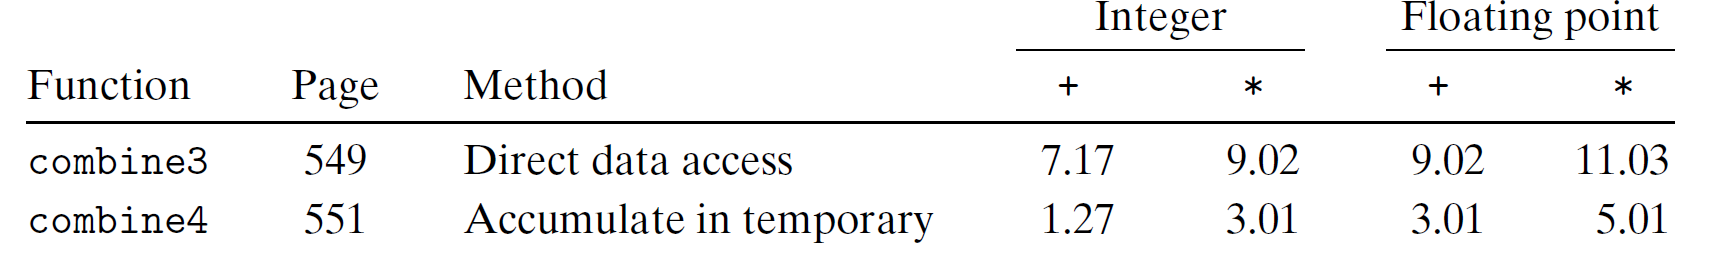
\includegraphics[scale=0.3]{pic/section5/pic4}
\end{figure}



\section{Understanding Modern Processors}

아몰랑


\section{Loop Unrolling}

while의 작동방식을 어셈블리로 한번보면 
if와  goto를 합쳐놓은 방식이다.
if는 단일 연산에비해느림 따라서
if검사를 적게 하게하면(=반복되는 횟수를 줄이면) 성능개선이 이루어진다.

\begin{lstlisting}[style = CStyle]
/* 2 x 1 loop unrolling */
void combine5(vec_ptr v, data_t *dest)
    {
    long i;
    long length = vec_length(v);
    long limit = length-1;
    data_t *data = get_vec_start(v);
    data_t acc = IDENT;

    /* Combine 2 elements at a time */
    for (i = 0; i < limit; i+=2) {
    acc = (acc OP data[i]) OP data[i+1];
    }

    /* Finish any remaining elements */
    for (; i < length; i++) {
    acc = acc OP data[i];
    }
    *dest = acc;
}
\end{lstlisting}


\begin{figure}[h!]
    \centering
    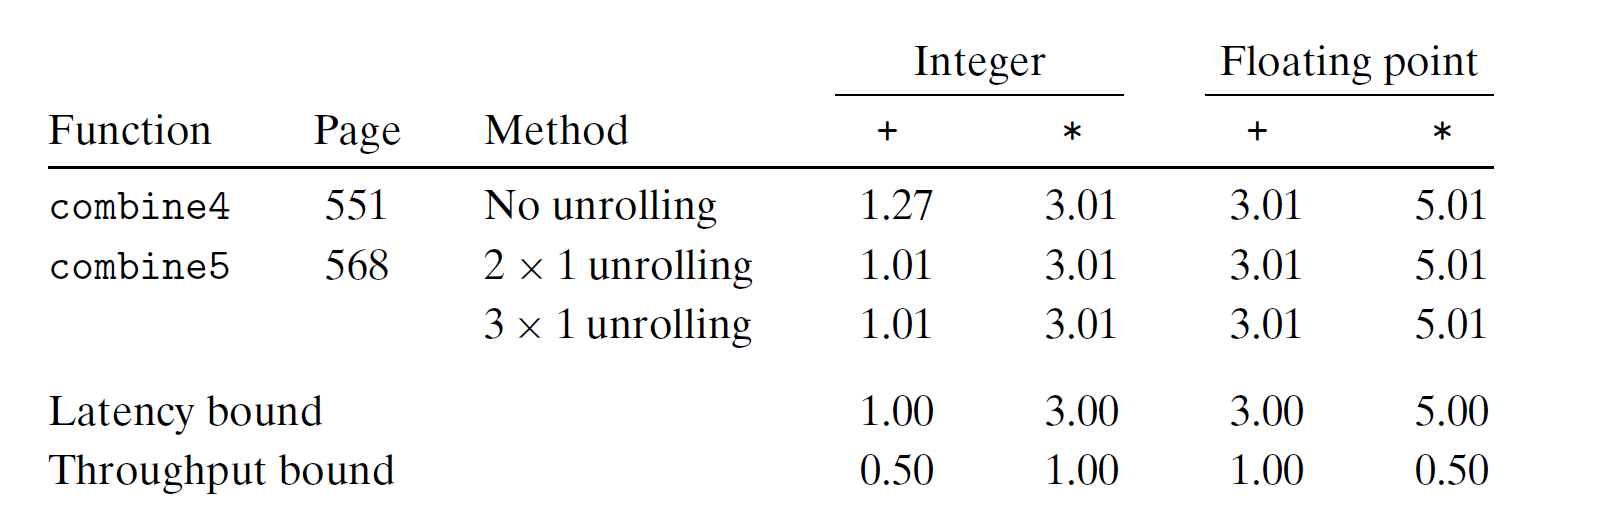
\includegraphics[scale=0.3]{pic/section5/pic5}
\end{figure}


\begin{figure}[h!]
    \centering
    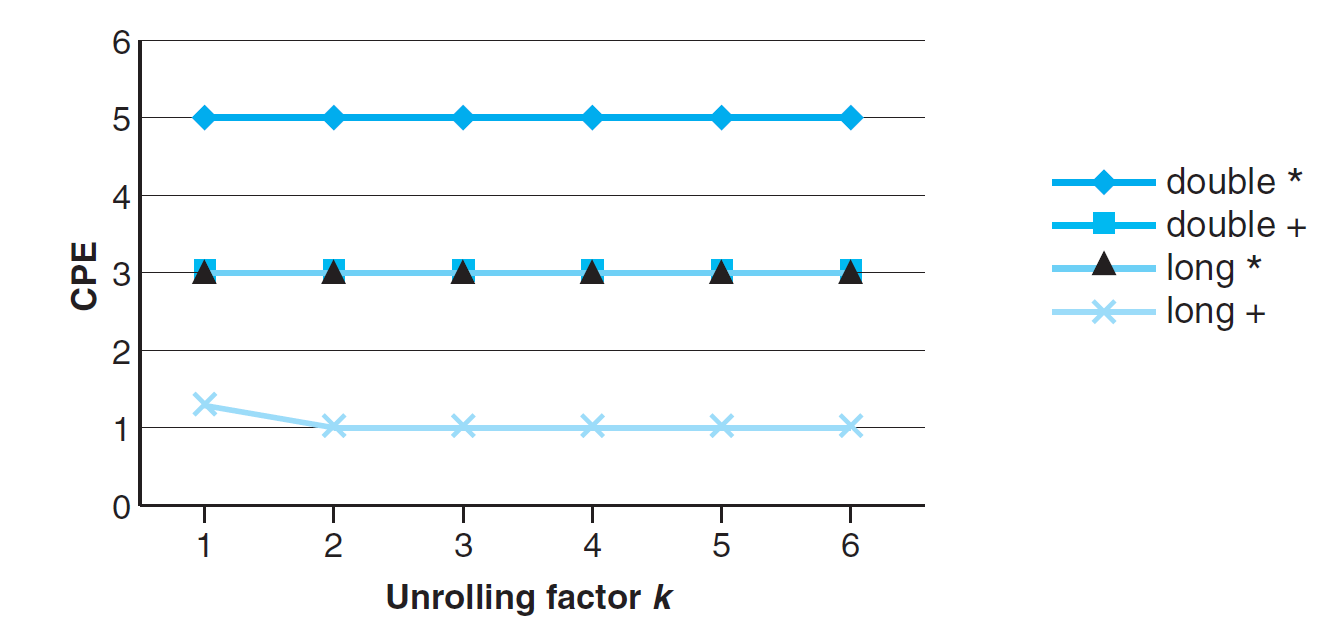
\includegraphics[scale=0.4]{pic/section5/pic6}
    \caption{ kx1 에따른 성능비교}
\end{figure}


이 생각을 할수있다.
루프풀기를 최대로하면 제일 좋은게아닌가?

여러단점이있다.

\url{http://z3moon.com/프로그래밍/loop_unrolling}

\url{https://en.wikipedia.org/wiki/Loop_unrolling}

\begin{enumerate}
    \item 코드 크기 증가
    \item 가독성 저해
    \item 함수호출이 있을 경우 캐시 미스율 향상
\end{enumerate}

연산이 복잡해질수록 인덱스의 계산과 if조건이 수행시간에 영향을 주지않는다.
for문 내부가 간단한 코드일때 가장 효과가 좋다.

\section{Enhancing Parallelism}

\subsubsection{Multiple Accumulators}
연산을 나눠서 계산하고 마지막에 합치는 방식

\begin{lstlisting}[style = CStyle]
/* 2 x 2 loop unrolling */
void combine6(vec_ptr v, data_t *dest)
{
    long i;
    long length = vec_length(v);
    long limit = length-1;
    data_t *data = get_vec_start(v);
    data_t acc0 = IDENT;
    data_t acc1 = IDENT;

    /* Combine 2 elements at a time */
    for (i = 0; i < limit; i+=2) {
    acc0 = acc0 OP data[i];
    acc1 = acc1 OP data[i+1];
    }

    /* Finish any remaining elements */
    for (; i < length; i++) {
    acc0 = acc0 OP data[i];
    }
    *dest = acc0 OP acc1;
}
\end{lstlisting}

\begin{figure}[h!]
    \centering
    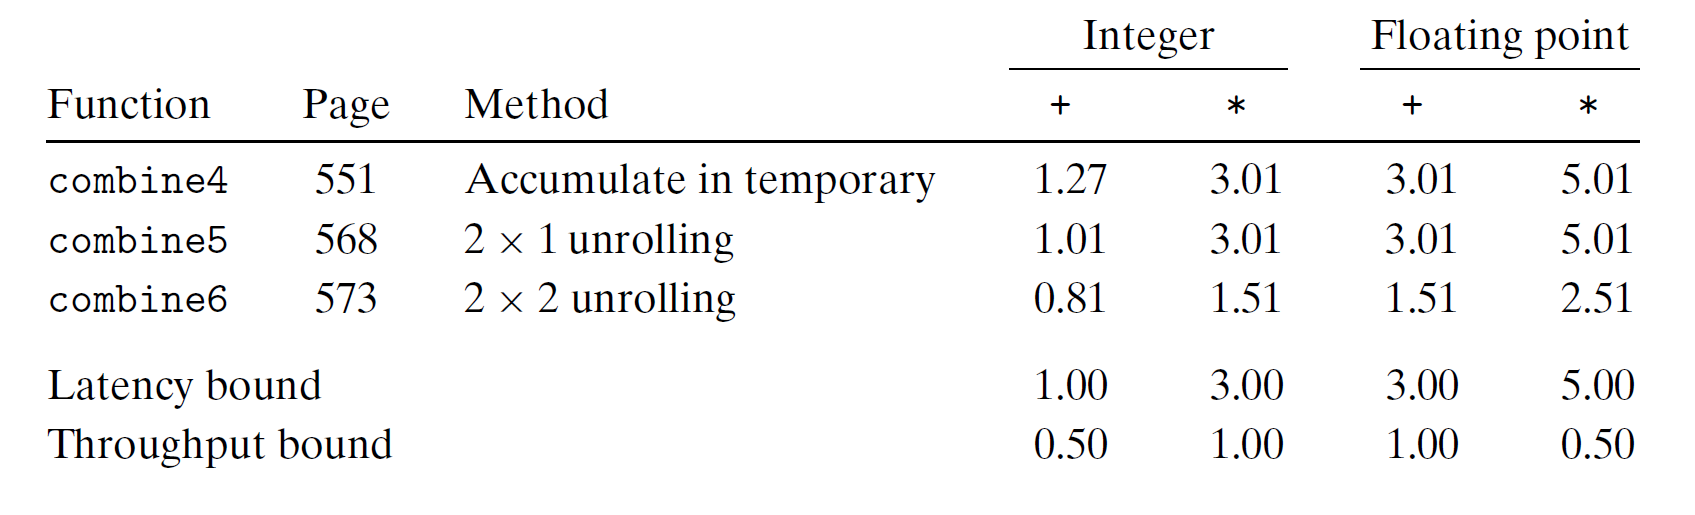
\includegraphics[scale=0.3]{pic/section5/pic7}
\end{figure}



\begin{figure}[h!]
    \centering
    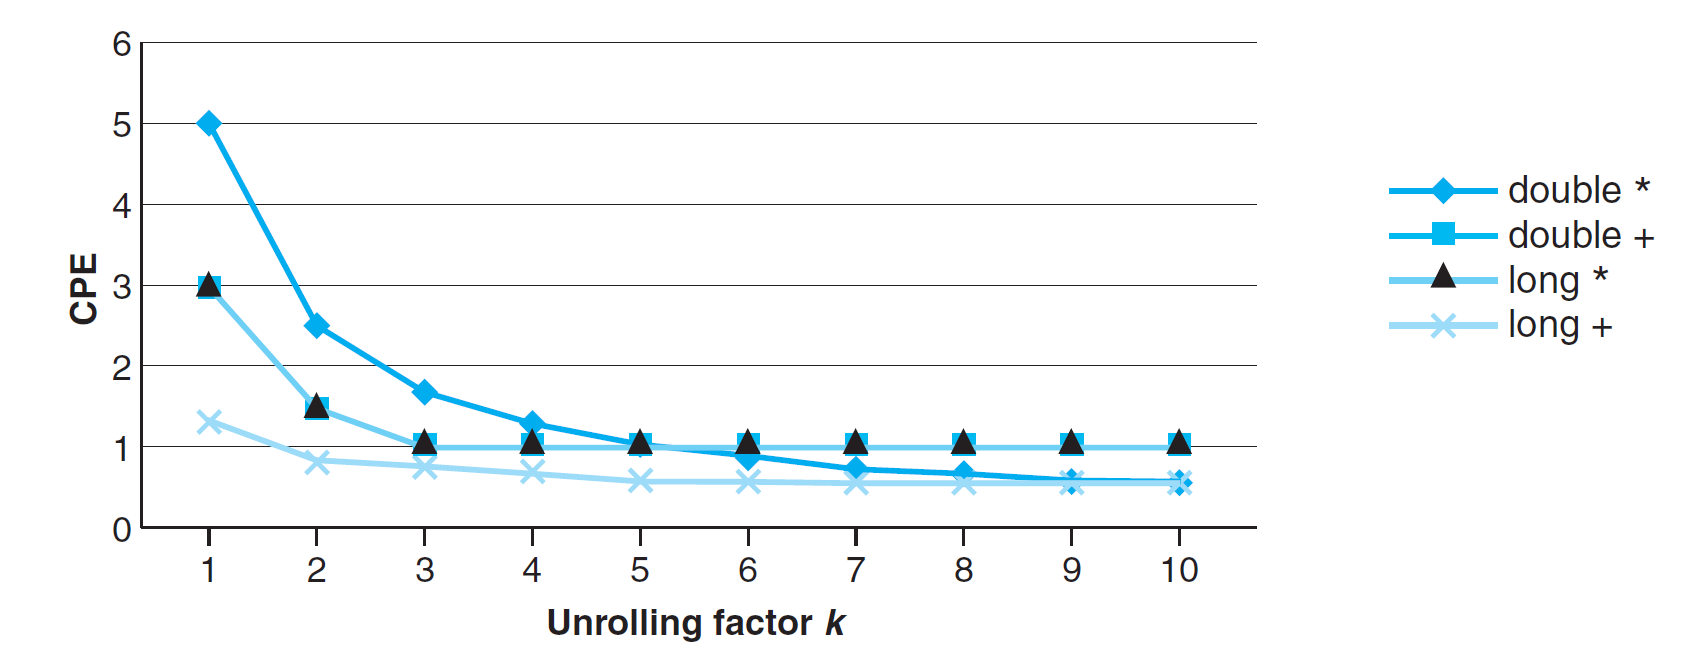
\includegraphics[scale=0.3]{pic/section5/pic8}
    \caption{kxk}
\end{figure}


\subsubsection{Reassociation Transformation}


\begin{lstlisting}[style = CStyle]
/* 2 x 1a loop unrolling */
void combine7(vec_ptr v, data_t *dest)
{
long i;
long length = vec_length(v);
long limit = length-1;
data_t *data = get_vec_start(v);
data_t acc = IDENT;

/* Combine 2 elements at a time */
for (i = 0; i < limit; i+=2) {
acc = acc OP (data[i] OP data[i+1]);
}

/* Finish any remaining elements */
for (; i < length; i++) {
acc = acc OP data[i];
}
*dest = acc;
}
\end{lstlisting}

combine5의 다음코드를


\begin{lstlisting}[style = CStyle]
    acc = (acc OP data[i]) OP data[i+1];
\end{lstlisting}


\begin{lstlisting}[style = CStyle]
    acc = acc OP (data[i] OP data[i+1]);
\end{lstlisting}
로 바꾼다.

\begin{figure}[h!]
    \centering
    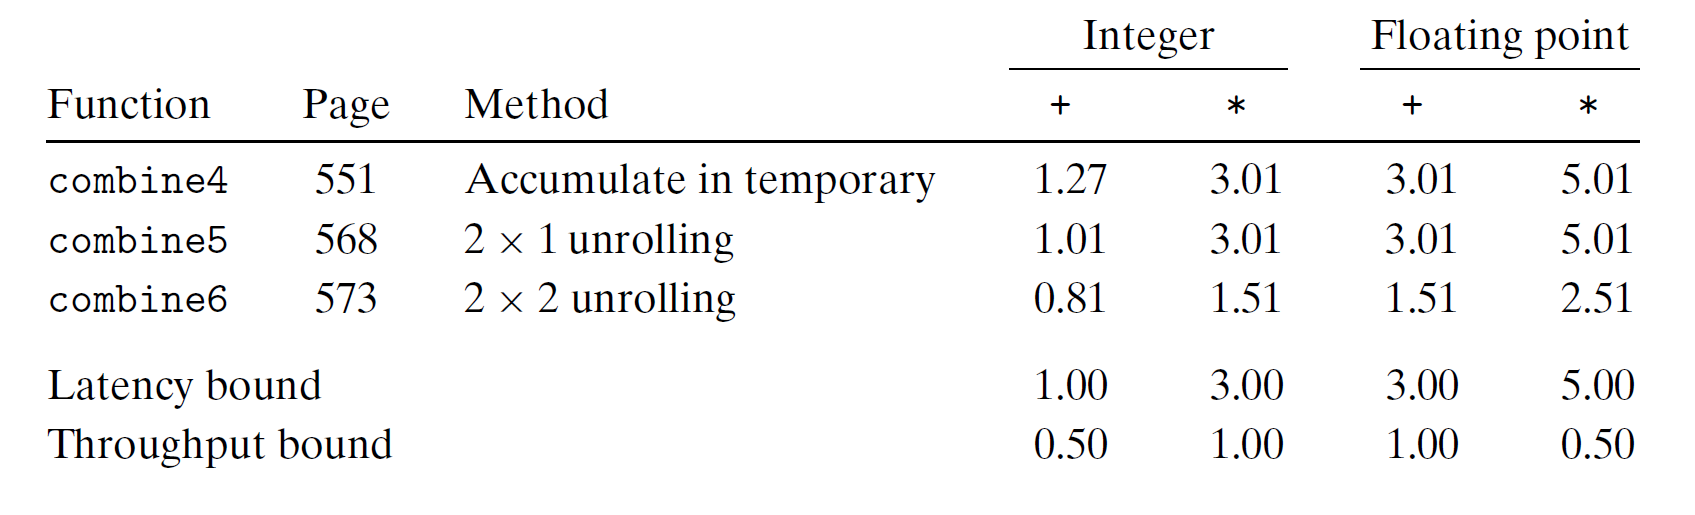
\includegraphics[scale=0.3]{pic/section5/pic7}
    \caption{}
\end{figure}



\begin{figure}[h!]
    \centering
    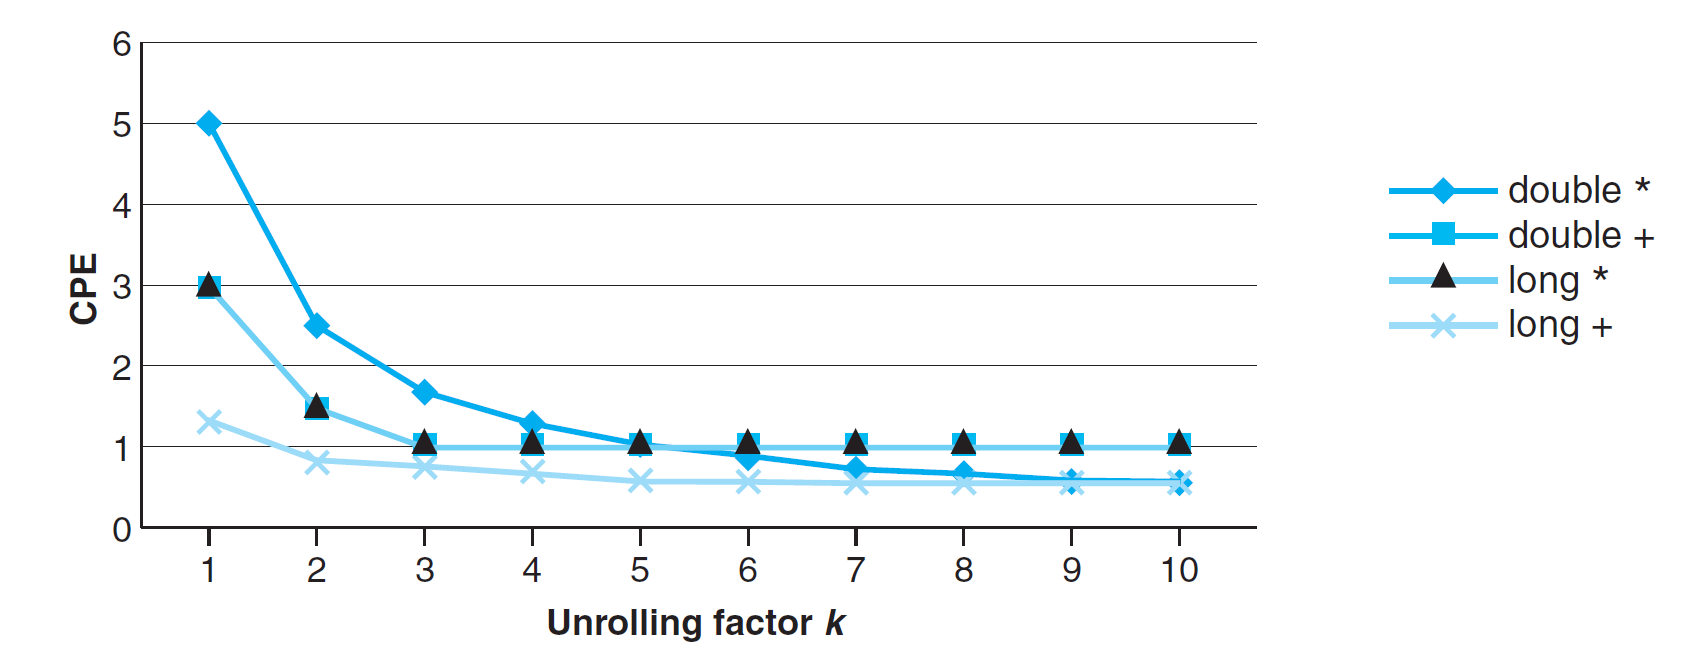
\includegraphics[scale=0.3]{pic/section5/pic8}
    \caption{}
\end{figure}




\chapter{}
% 6
% The Memory Hierarchy 615
% 6.1 Storage Technologies 617
% 6.2 Locality 640
% 6.3 The Memory Hierarchy 645
% 6.4 Cache Memories 650
% 6.5 Writing Cache-Friendly Code 669
% 6.6 Putting It Together: The Impact of Caches on Program Performance 675
% 6.7 Summary 684
% Bibliographic Notes 684
% Homework Problems 685
% Solutions to Practice Problems 696


\part{ Running Programs on a System}


\chapter{Linker}

\section{Compiler Drivers}



\begin{lstlisting}[language=bash]
    linux> gcc -Og -o prog main.c sum.css

    cpp [other arguments] main.c /tmp/main.is
    as [other arguments] -o /tmp/main.o /tmp/main.s
    ld -o prog [system object files and args] /tmp/main.o /tmp/sum.o
    linux> ./prog
\end{lstlisting}

\begin{figure}[h!]
    \centering
    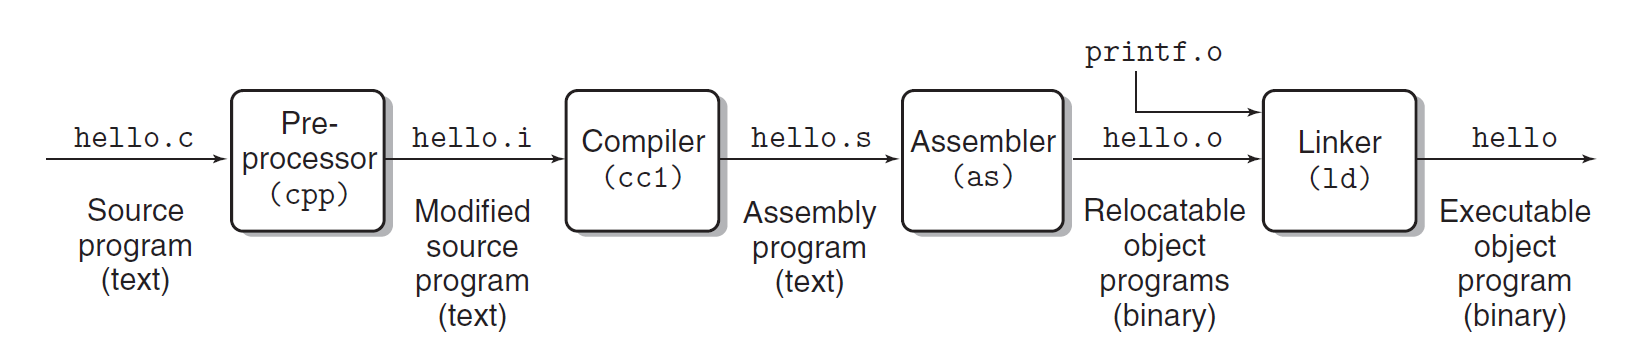
\includegraphics[scale=0.5]{pic/section7/pic1.png}
    \caption{Static linking. The linker combines relocatable    object files to form an executable object file prog}
\end{figure}



\section{Static Linking}

about sympbol(7.5)
\begin{enumerate}
    \item symbol resolution(7.6)
    \item Relocation(7.7)
\end{enumerate}

\section{Object Files}

Object files are merely collections of blocks
of bytes. Some of these blocks contain program code, others contain program
data, and others contain data structures that guide the linker and loader. A linker
concatenates blocks together, decides on run-time locations for the concatenated
blocks, and modifies various locations within the code and data blocks. Linkers
have minimal understanding of the target machine. The compilers and assemblers
that generate the object files have already done most of the work.


\begin{itemize}
    \item Relocatable ob~(7.4) : compiler,assembler output
    \item Executable ob~(7.8,7.9) linker output
    \item shared ob~ (7.10)
\end{itemize}



\section{Relocatable Object Files}


\begin{figure}[h!]
    \centering
    \includegraphics[scale=0.5]{pic/section7/pic2.png}
    \caption{Typical ELF relocatable object file.}
\end{figure}


\section{Symbols and Symbol Tables}


\begin{itemize}
    \item Global symbols that are defined by module m and that can be referenced by other modules :nonstatic C functions and
    global variables
    \item Global symbols that are referenced by module m but defined by some other module : nonstatic C functions and global variables that are defined in other modules.
    \item Local symbolsthat are defined and referenced exclusively by module m : nonstatic C functions and global variables that are defined in other modules.
\end{itemize}

\section{Symbol Resolution}

\subsection{How Linkers Resolve Duplicate Symbol Name}

\begin{itemize}
    \item strong symbol : 초기화된 전역변수
    \item weak symbol : 초기화x 전역변수
\end{itemize}

Rule
\begin{enumerate}
    \item Multiple strong symbols with the same name are not allowed.
    \item Given a strong symbol and multiple weak symbols with the same name, choose the strong symbol.
    \item Given multiple weak symbols with the same name, choose any of the weak symbols.
\end{enumerate}

\subsection{Linking with Static Libraries}

라이브러리 생성

\begin{lstlisting}[language=bash]
linux> gcc -c addvec.c multvec.c
linux> ar rcs libvector.a addvec.o multvec.o
\end{lstlisting}

라이브러리 링킹

\begin{lstlisting}[language=bash]
    
linux> gcc -c main2.c
linux> gcc -static -o prog2c main2.o ./libvector.a

linux> gcc -c main2.c
linux> gcc -static -o prog2c main2.o -L. -lvector

\end{lstlisting}

\begin{figure}[h!]
    \centering
    \includegraphics[scale=0.5]{pic/section7/pic3.png}
    \caption{Linking with static libraries.}
\end{figure}




\section{Relocation}

\begin{enumerate}
    \item Relocating sections and symbol definitionss   인스트럭션과 전역변수들이 런타임 메모리 주소를 가진다.
    \item Relocating symbol references within sections.    
    모든 심볼들이 런타임 메모리 주소를 가진다.
\end{enumerate}

\subsection{Relocation Entries}
위치를 모르는 심볼을 어떻게 처리할지에대해 어셈블러가만듬


재배치타입

\begin{itemize}
    \item R\_X86\_64\_PC32
    \item R\_X86\_64\_32.
\end{itemize}

\subsection{Relocating Symbol References}


\section{Executable Object Files}


\begin{figure}[h!]
    \centering
    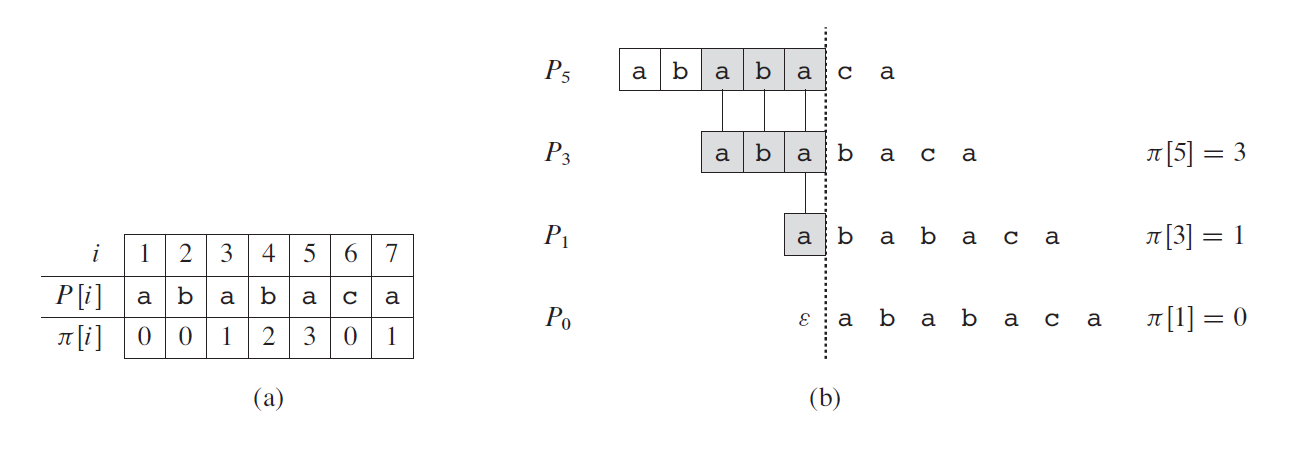
\includegraphics[scale=0.4]{pic/section7/pic4.png}
    \caption{Typical ELF executable object file.}
\end{figure}

\section{Loading Executable Object Files}

\begin{figure}[h!]
    \centering
    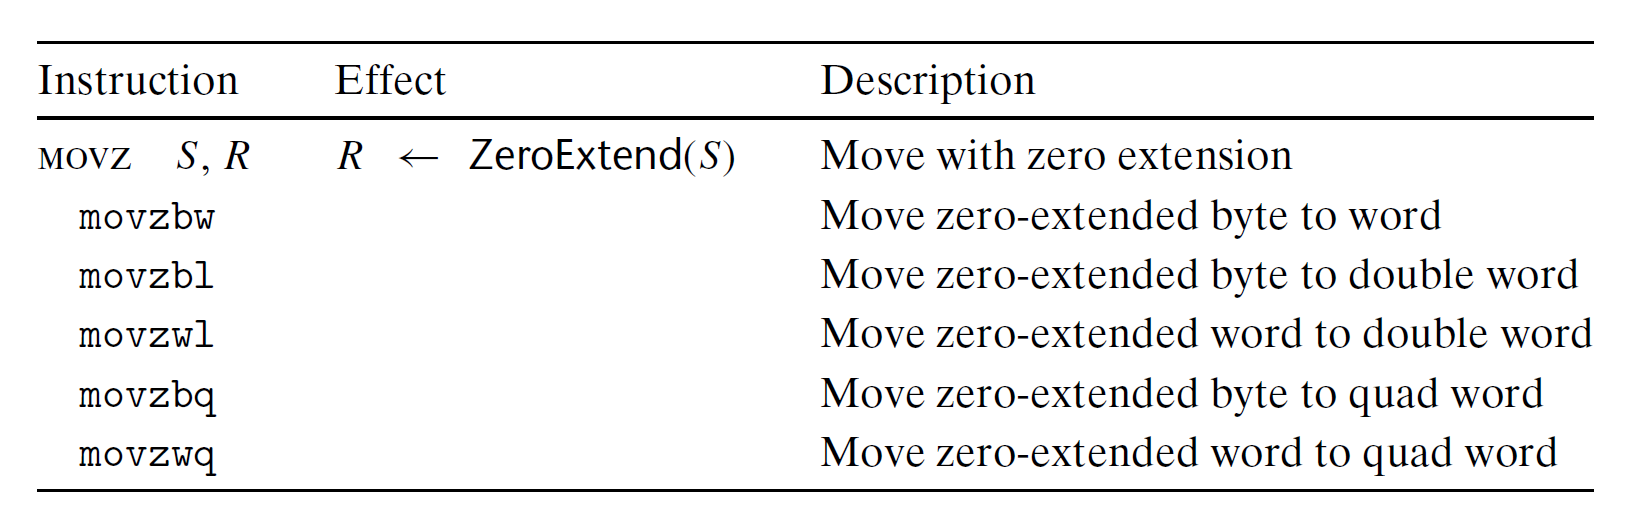
\includegraphics[scale=0.5]{pic/section7/pic5.png}
    \caption{\textbf{Linux x86-64 run-time memory image.} 
    Gaps due to segment alignment requirements and addressspace layout randomization (ASLR) are not shown. Not to scale}
\end{figure}

loading : 실행가능한 목적파일 내의 코드와 데이터를 메모리로 복사하고 첫번째 인스트럭션(엔트리 포인트)으로 점프해서실행하는 과정

\section{Dynamic Linking with Shared Libraries}

\begin{lstlisting}[language=bash]
linux> gcc -shared -fpic -o libvector.so addvec.c multvec.c
\end{lstlisting}

\begin{lstlisting}[language=bash]
    linux> gcc -o prog2l main2.c ./libvector.so
\end{lstlisting}

\begin{figure}[h!]
    \centering
    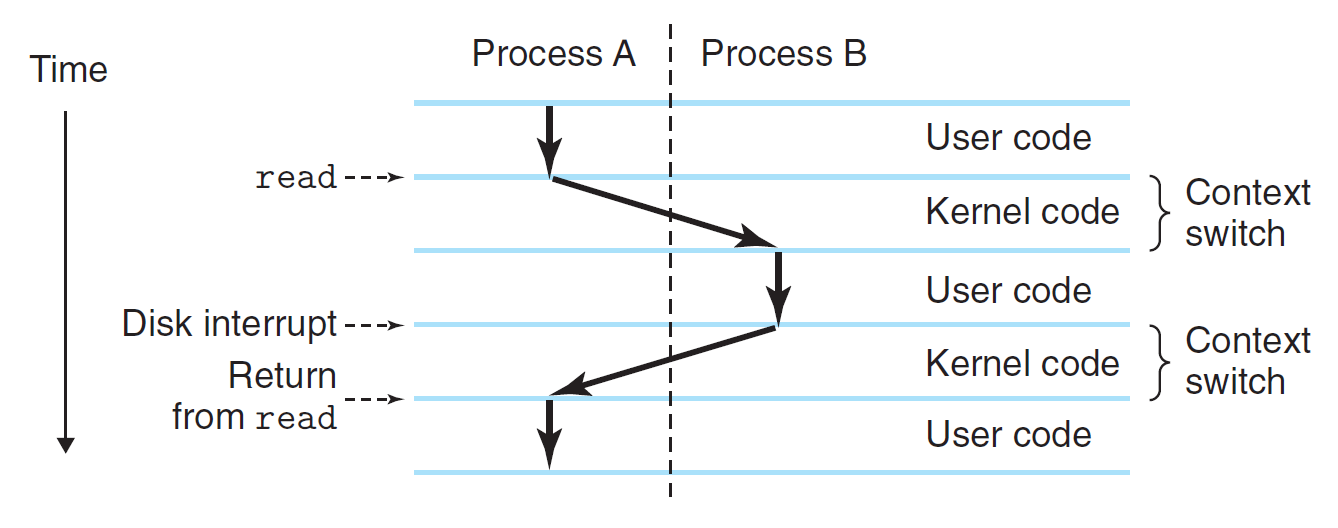
\includegraphics[scale=0.5]{pic/section7/pic6.png}
    \caption{Dynamic linking with shared libraries.}
\end{figure}



\section{Loading and Linking Shared Libraries from Applications}

\section{Position-Independent Code (PIC)}


\section{Library Interpositioning}


% \chapter{Linking}

% 7.1 Compiler Drivers 707
% 7.2 Static Linking 708
% 7.3 Object Files 709
% 7.4 Relocatable Object Files 710
% 7.5 Symbols and Symbol Tables 711
% 7.6 Symbol Resolution 715
% 7.7 Relocation 725
% 7.8 Executable Object Files 731
% 7.9 Loading Executable Object Files 733
% 7.10 Dynamic Linking with Shared Libraries 734
% 7.11 Loading and Linking Shared Libraries from Applications 737
% 7.12 Position-Independent Code (PIC) 740
% 7.13 Library Interpositioning 743
% 7.14 Tools for Manipulating Object Files 749
% 7.15 Summary 749
% Bibliographic Notes 750
% Homework Problems 750
% Solutions to Practice Problems 753


\chapter{Exceptional Control Flow}

\section{Exceptions}

이벤트 발생시에 예외 테이블이라고하는 점프 테이블을 통해서 운영체제에서 핸들러로 프로시저 콜을 하게한다.
그후에 제어를 다음 세가지중 하나로 처리한다.

\begin{enumerate}
    \item 현재 인스트럭션에 돌려준다
    \item 다음 인스트럭션으로 돌려준다 
    \item 프로그램을 종료한다.
\end{enumerate}

예외에는 하드웨어,소프트웨어 사이에서 각각 일어날 수 있으며 각각의 프로세서,OS 설계자가 예외를 미리 정해놓고 시스템 부팅시에 점프테이블에 할당하여 쓰는식.

예외 종류
\begin{itemize}
    \item inturrupt(비동기) : I/O에서 시그널  다음 인스트럭션으로 돌려준다.
    \item trap(동기) : instruction 실행결과. syscall로 OS단에서 처리,다음 인스트럭션으로 돌려준다.
    \item fault(동기) : ex) 가상 메모리 페이지 오류, 현재 인스트럭션으로 돌려준다.
    \item abort(동기) : 하드웨어 단의 복구불가능 에러, 프로그램 종료
\end{itemize}

syscall : 

리눅스에서 제공하는 syscall
\begin{itemize}
    \item read
    \item write
    \item open
    \item close
    \item stat
    \item mmap
    \item brk
    \item dup2
    \item pause
    \item alarm
    \item getpid
    \item fork
    \item execve
    \item \_exit
    \item sait4
    \item kill
\end{itemize}


\section{Processes}

프로세스 생성에는 두가지 종류가있다.

리눅스 프로세스 제어는 unistd.h에 함수가 정의되어 있다.
\begin{itemize}
    \item fork : 새로운 메모리에 매핑하여 자식프로세스로서 호출
    \item exevce : 현재 실행되는 프로그램의 메모리에 덮어쓰워 프로세스를 호출
\end{itemize}

exevce는 실행할 프로그램에 argv(인자리스트)와  envp(환경변수)를 보낼수있다

\begin{figure}[h!]
    \centering
    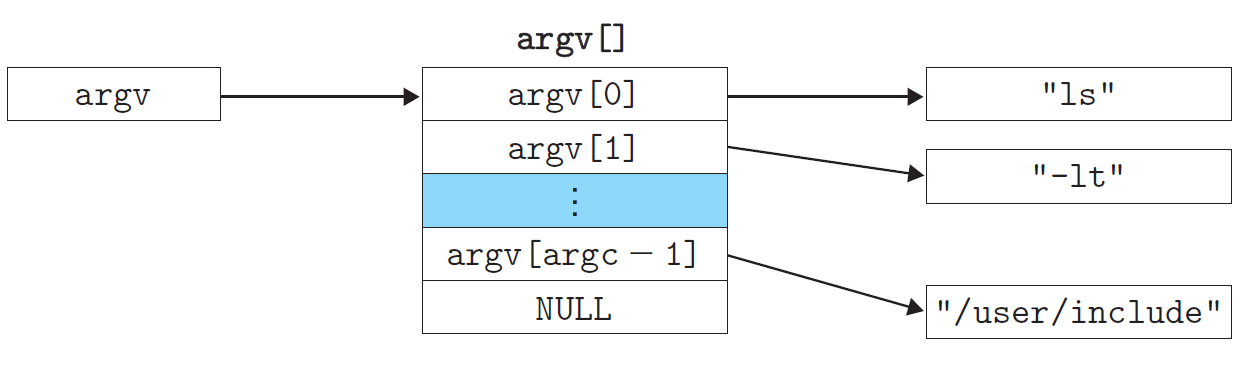
\includegraphics[scale=0.5]{pic/section8/pic1}
    \caption{Organization of an argument list.}
\end{figure}


\begin{figure}[h!]
    \centering
    \includegraphics[scale=0.47]{pic/section8/pic2}
    \caption{Organization of an environment variable list.}
\end{figure}

\begin{figure}[h!]
    \centering
    \includegraphics[scale=0.5]{pic/section8/pic3}
    \caption{Typical organization of the user stack when a    new program starts.}
\end{figure}



\section{Signals}


\section{Nonlocal Jumps}

setjmp longjmp

\section{Tools for Manipulating Processes}



% --------------------------------------------------
% 8
% \chapter{Exceptional Control Flow}
% 8.1 Exceptions 759
% 8.1.1 Exception Handling 760
% 8.1.2 Classes of Exceptions 762
% 8.1.3 Exceptions in Linux/x86-64 Systems 765
% 8.2 Processes 768
% 8.2.1 Logical Control Flow 768
% 8.2.2 Concurrent Flows 769
% 8.2.3 Private Address Space 770
% 8.2.4 User and Kernel Modes 770
% 8.2.5 Context Switches 772
% 8.3 System Call Error Handling 773
% 8.4 Process Control 774
% 8.4.1 Obtaining Process IDs 775
% 8.4.2 Creating and Terminating Processes 775
% 8.4.3 Reaping Child Processes 779
% 8.4.4 Putting Processes to Sleep 785
% 8.4.5 Loading and Running Programs 786
% 8.4.6 Using fork and execve to Run Programs 789
% 8.5 Signals 792
% 8.5.1 Signal Terminology 794
% 8.5.2 Sending Signals 795
% 8.5.3 Receiving Signals 798
% 8.5.4 Blocking and Unblocking Signals 800
% 8.5.5 Writing Signal Handlers 802
% 8.5.6 Synchronizing Flows to Avoid Nasty Concurrency Bugs 812
% 8.5.7 Explicitly Waiting for Signals 814
% 8.6 Nonlocal Jumps 817
% 8.7 Tools for Manipulating Processes 822
% 8.8 Summary 823
% Bibliographic Notes 823
% Homework Problems 824
% Solutions to Practice Problems 831



% \chapter{Virtual Memory}

% 9.1 Physical and Virtual Addressing 839
% 9.2 Address Spaces 840
% 9.3 VM as a Tool for Caching 841
% 9.3.1 DRAM Cache Organization 842
% 9.3.2 Page Tables 842
% 9.3.3 Page Hits 844
% 9.3.4 Page Faults 844
% 9.3.5 Allocating Pages 846
% 9.3.6 Locality to the Rescue Again 846
% 9.4 VM as a Tool for Memory Management 847
% 9.5 VM as a Tool for Memory Protection 848
% 9.6 Address Translation 849
% 9.6.1 Integrating Caches and VM 853
% 9.6.2 Speeding Up Address Translation with a TLB 853
% 9.6.3 Multi-Level Page Tables 855
% 9.6.4 Putting It Together: End-to-End Address Translation 857
% 9.7 Case Study: The Intel Core i7/Linux Memory System 861
% 9.7.1 Core i7 Address Translation 862
% 9.7.2 Linux Virtual Memory System 864
% 9.8 Memory Mapping 869
% 9.8.1 Shared Objects Revisited 869
% 9.8.2 The fork Function Revisited 872
% 9.8.3 The execve Function Revisited 872
% 9.8.4 User-Level Memory Mapping with the mmap Function 873
% 9.9 Dynamic Memory Allocation 875
% 9.9.1 The malloc and free Functions 876
% 9.9.2 Why Dynamic Memory Allocation? 879
% 9.9.3 Allocator Requirements and Goals 880
% 9.9.4 Fragmentation 882
% 9.9.5 Implementation Issues 882
% 9.9.6 Implicit Free Lists 883
% 9.9.7 Placing Allocated Blocks 885
% 9.9.8 Splitting Free Blocks 885
% 9.9.9 Getting Additional Heap Memory 886
% 9.9.10 Coalescing Free Blocks 886
% 9.9.11 Coalescing with Boundary Tags 887
% 9.9.12 Putting It Together: Implementing a Simple Allocator 890
% 9.9.13 Explicit Free Lists 898
% 9.9.14 Segregated Free Lists 899
% 9.10 Garbage Collection 901
% 9.10.1 Garbage Collector Basics 902
% 9.10.2 Mark&Sweep Garbage Collectors 903
% 9.10.3 Conservative Mark&Sweep for C Programs 905
% 9.11 Common Memory-Related Bugs in C Programs 906
% 9.11.1 Dereferencing Bad Pointers 906
% 9.11.2 Reading Uninitialized Memory 907
% 9.11.3 Allowing Stack Buffer Overflows 907
% 9.11.4 Assuming That Pointers and the Objects They Point to
% Are the Same Size 908
% 9.11.5 Making Off-by-One Errors 908
% 9.11.6 Referencing a Pointer Instead of the Object It Points To 909
% 9.11.7 Misunderstanding Pointer Arithmetic 909
% 9.11.8 Referencing Nonexistent Variables 910
% 9.11.9 Referencing Data in Free Heap Blocks 910
% 9.11.10 Introducing Memory Leaks 911
% 9.12 Summary 911
% Bibliographic Notes 912
% Homework Problems 912
% Solutions to Practice Problems 916
% Part III Interaction and Communication
% between Programs


\part{ Interaction and Communication between Programs}




% \chapter{System-Level I/O}

% 10.1 Unix I/O 926
% 10.2 Files 927
% 10.3 Opening and Closing Files 929
% 10.4 Reading and Writing Files 931
% 10.5 Robust Reading and Writing with the Rio Package 933
% 10.5.1 Rio Unbuffered Input and Output Functions 933
% 10.5.2 Rio Buffered Input Functions 934
% 10.6 Reading File Metadata 939
% 10.7 Reading Directory Contents 941
% 10.8 Sharing Files 942
% 10.9 I/O Redirection 945
% 10.10 Standard I/O 947
% 10.11 Putting It Together: Which I/O Functions Should I Use? 947
% 10.12 Summary 949
% Bibliographic Notes 950
% Homework Problems 950
% Solutions to Practice Problems 951

% \chapter{Network Programming}
% 11.1 The Client-Server Programming Model 954
% 11.2 Networks 955
% 11.3 The Global IP Internet 960
% 11.3.1 IP Addresses 961
% 11.3.2 Internet Domain Names 963
% 11.3.3 Internet Connections 965
% 11.4 The Sockets Interface 968
% 11.4.1 Socket Address Structures 969
% 11.4.2 The socket Function 970
% 11.4.3 The connect Function 970
% 11.4.4 The bind Function 971
% 11.4.5 The listen Function 971
% 11.4.6 The accept Function 972
% 11.4.7 Host and Service Conversion 973
% 11.4.8 Helper Functions for the Sockets Interface 978
% 11.4.9 Example Echo Client and Server 980
% 11.5 Web Servers 984
% 11.5.1 Web Basics 984
% 11.5.2 Web Content 985
% 11.5.3 HTTP Transactions 986
% 11.5.4 Serving Dynamic Content 989
% 11.6 Putting It Together: The Tiny Web Server 992
% 11.7 Summary 1000
% Bibliographic Notes 1001
% Homework Problems 1001
% Solutions to Practice Problems 1002

% \chapter{Concurrent Programming}
% 12.1 Concurrent Programming with Processes 1009
% 12.1.1 A Concurrent Server Based on Processes 1010
% 12.1.2 Pros and Cons of Processes 1011
% 12.2 Concurrent Programming with I/O Multiplexing 1013
% 12.2.1 A Concurrent Event-Driven Server Based on I/O
% Multiplexing 1016
% 12.2.2 Pros and Cons of I/O Multiplexing 1021
% 12.3 Concurrent Programming with Threads 1021
% 12.3.1 Thread Execution Model 1022
% 12.3.2 Posix Threads 1023
% 12.3.3 Creating Threads 1024
% 12.3.4 Terminating Threads 1024
% 12.3.5 Reaping Terminated Threads 1025
% 12.3.6 Detaching Threads 1025
% 12.3.7 Initializing Threads 1026
% 12.3.8 A Concurrent Server Based on Threads 1027
% 12.4 Shared Variables in Threaded Programs 1028
% 12.4.1 Threads Memory Model 1029
% 12.4.2 Mapping Variables to Memory 1030
% 12.4.3 Shared Variables 1031
% 12.5 Synchronizing Threads with Semaphores 1031
% 12.5.1 Progress Graphs 1035
% 12.5.2 Semaphores 1037
% 12.5.3 Using Semaphores for Mutual Exclusion 1038
% 12.5.4 Using Semaphores to Schedule Shared Resources 1040
% 12.5.5 Putting It Together: A Concurrent Server Based on
% Prethreading 1044
% 12.6 Using Threads for Parallelism 1049
% 12.7 Other Concurrency Issues 1056
% 12.7.1 Thread Safety 1056
% 12.7.2 Reentrancy 1059
% 12.7.3 Using Existing Library Functions in Threaded Programs 1060
% 12.7.4 Races 1061
% 12.7.5 Deadlocks 1063
% 12.8 Summary 1066
% Bibliographic Notes 1066
% Homework Problems 1067
% Solutions to Practice Problems 1072

\end{document}